\documentclass{standalone}
\usepackage{tikz}
\usepackage{ctex,siunitx}
\setCJKmainfont{Noto Serif CJK SC}
\usepackage{tkz-euclide}
\usepackage{amsmath}
\usetikzlibrary{patterns, calc,3d}
\usetikzlibrary {decorations.pathmorphing,decorations.pathreplacing,decorations.shapes}
\begin{document}
\small
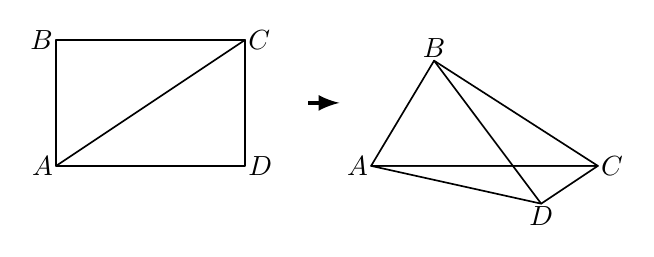
\begin{tikzpicture}[>=latex,scale=0.8,inner sep=1pt]
  \tkzDefPoints{0/0/A,3/0/D,3/2/C,0/2/B}
  \tkzDrawPolygon[semithick](A,B,C,D)
  \tkzDrawSegments[semithick](A,C)
  \tkzLabelPoints[left](A,B)
  \tkzLabelPoints[right](C,D)
  \draw[ultra thick,->](4,1)--++(0.5,0);
  \begin{scope}[xshift=5cm]
    \tkzDefPoints{0/0/A,1/1.67/B,3.6/0/C,2.7/-0.6/D}
    \tkzDrawPolygon[semithick](A,B,C)
    \tkzDrawPolygon[semithick](A,C,D)
    \tkzDrawSegments[semithick](B,D)
    \tkzLabelPoints[left](A)
    \tkzLabelPoints[right](C)
    \tkzLabelPoints[above](B)
    \tkzLabelPoints(D)
  \end{scope}
\end{tikzpicture}
\end{document}